\chapter{A programról}
\label{ch:about_hestia}

\section{Motiváció}

Felmerülhet a kérdés, hogy pontosan miért van szükség jelen esetben egy új programra -- git-ből kinyerhetőek a vizsgálathoz szükséges statisztikák akár csak egy egyszerű bash script segítségével, a coverage adatokat pedig a már amúgy is generált report-ból szemre meg tudjuk vizsgálni.

Egyrészt a triviális és sok szoftverfejlesztési projekt motivációjaként szolgáló válasz itt is a kényelem és automatizálás. Természetesen lehet bash script-eket használni, kézzel feldolgozni a kimenetüket, majd szemmel összenézni azt egy tetszőleges formátumú coverage report-al, de ez nem éppen ideális felhasználása egy fejlesztő idejének, főleg nem akkor, ha ezt sokszor meg kell ismételni.

Másrészt fontos megjegyezni, hogy ugyan specifikusan a vizsgálat számára releváns git statisztikák követésére léteznek megoldások (nevezetesen például a korábban már említett \citeauthor{tornhillXrays} által fejlesztett, fizetős CodeScene\footnote{CodeScene: https://codescene.io/}, illetve az annál sokkal egyszerűbb GitNStats\footnote{GitNStats: https://github.com/rubberduck203/GitNStats}), ezen megoldások azonban nem használják ki a coverage által nyújtott extra lehetőségeket.

\section{Architektúra}

A program, ami a Hestia becenevet kapta, két nagy részből áll:
\begin{enumerate}
    \item Hestia: a teljes modellt ábrázoló, perzisztáló és a kliens felé kiszolgáló .NET 5 alapokon írt program
    \item Hestia-UI\footnote{Forráskód: https://github.com/marczinusd/hestia-ui}: Angular 11-ben írt vékony kliens ami REST API-n keresztül kéri le a .NET-es web service-től az adatbázisba mentett repository-kat
\end{enumerate}

\section{A modell}

Mielőtt részletesen ismeretetném a programokat, előbb fontos tisztázni a koncepciókat és terminológiákat, amikre a projekt mindkét rétege épít. A bevezetésben elhangzott egy rövid bevezetés a git verziókövetőbe és a unit teszt coverage-be, illetve említésre került, hogy a jelen végzett analízis szempontjából nagyon hasonló absztrakciókkal dolgozik mindkettő.

A modell legmagasabb szintű absztrakciója maga a repository: ez értelemszerűen egy projekt teljes forráskódjának a git-ben való leképezése.

Közvetlen a repository-hoz alatt lévő absztrakció az úgynevezett snapshot. Ezalatt egy repository egy adott commit-jánál megfigyelt állapotot értjük. Maga a git nem értelmezi pontosan ezt a koncepciót, illetve a coverage report-ok szempontjából is ekvivalens gyakorlatban egy snapshot és egy repository, mégis érdemes tisztázni, hogy pontosan mit jelent, mert a későbbiekben fontos lesz, hogy egy repository állapotát több, hozzá tartozó snapshot-on keresztül figyeljük meg.

A snapshot-okhoz közvetlen kapcsolódik fájlok egy halmaza. Ez az első réteg, amit mind a git, mind egy coverage report definiál. Itt fontos megjegyezni a statisztikákat, amiket a program képes kinyerni fájl-szinten:
\begin{enumerate}
    \item Egyedi szerzők száma
    \item Commit-ok száma, amik tartalmazták az adott fájlt
    \item Fájl-szintű coverage arány
\end{enumerate}

A modell legalsó rétegét egy fájlban található forráskód sorai képezik. Egy sorhoz a program a következő statisztikákat társítja:
\begin{enumerate}
    \item Egyedi szerzők száma
    \item Commit-ok száma, amik értintették az adott sort
    \item Unit tesztek száma, amik értintették az adott sort
    \item Branch coverage
\end{enumerate}

A gyakorlatban a sorok statisztikái kiemelkedően hasznosak, hiszen betektintést adnak egy fájl kiemelkedően problémás részeire, ajánlást adva potenciális refactor-ra. Ebben a diplomamunkában végzett analízis szempontjából azonban a fájl-szintű statisztikák lesznek relevánsak, mivel mintákat próbálunk keresni teljesen ismeretlen kódbázisokban.

\section{Hestia - a backend modell}

Az előző szekcióban ismertetett modellt, illetve logikát implementálja a Hestia. A program .NET 5-ben készült, ami azt jelenti, hogy teljesen platformfüggetlen: tesztelve lett Windows 10, Linux és MacOS operációs rendszerek alatt. Itt fontos azonban megjegyezni, hogy bár a platformfüggetlenség garantált, a git természetéből fakadóan abszolút nem mindegy, hogy milyen operációs rendszeren futtatjuk a repository analíziseket, hiszen a git notóriusan lassú a Windows fájlrendszerein -- nagyságrendileg tízszer tovább fog tartani egy Windows-on futtatott analízis a Linux-on vagy MacOS-en futtatott analízissel szemben.

Maga a program stílusát tekintve funkcionális koncepciókra épít: kap egy bemeneti értékhalmazt és azokat tiszta függvényeken keresztül transzformálja addig, amíg egy coverage és git statisztikákkal rendekező snapshot-ot nem kapunk. Itt emelném ki a nagyszerű language-ext\footnote{language-ext: https://github.com/louthy/language-ext} nevű könyvtárat, ami a C\# funkcionális repertoárját egészíti ki, ezzel elősegítve a Hestia modelljének funkcionális tisztaságát.

A felépített modellt a program Entity Framework Core segítségével tetszőleges adatbázisban képes tárolni az eredményeket -- per pillanat SQLite-ra van konfigurálva a projekt a könnyű hordozhatóság és tesztelhetőség érdekében, de ez triviális mennyiségű munkával átírható a népszerűbb adatbázisok akármelyikére.

\section{Konzolos futtató}

A repository analízisek gyors, könnyen ismételhető futtatása kritikus követelménye volt a projektnek. Eleinte egy grafikus futtató felülettel kísérleteztem, de hamar kiderültek a hátrányai (nevezetesen az ismételhetőség volt problémás), így a konzolos futtatás maradt az egyetlen opció. Egy repository-ra mindössze egy relatíve egyszerű konfigurációs fájlt kell létrehozni az alábbi formátumban, amit a futtató végre tud hajtani:

\lstset{caption={A React projekt Hestia konfigurációja}, language=json, numberstyle=\small}
\begin{lstlisting}
{
  "$schema": "https://raw.githubusercontent.com/marczinusd/hestia/master/src/Hestia.ConsoleRunner/config.schema.json",
  "coverageReportLocation": "~/dev/react/coverage/lcov.info",
  "repoRoot": "~/dev/react",
  "sourceRelativePath": "packages",
  "fileExtensions": [".js", ".ts"],
  "statGranularity": "full",
  "ignorePatterns": [],
  "buildCommands": ["yarn install"],
  "testCommands": ["yarn test --coverage"]
}
\end{lstlisting}

Műveletigény szempontjából a konfigurációs fájl tartalmaz egy nagyon fontos paramétert \code{statGranularity}, ami lehet "full", vagy "file". Amennyiben file értéket kap, akkor csak fájl-szintű git statisztikákat generálunk, aminek a műveletigénye (élve azzal a feltételezéssel, hogy a git parancsok műveletigényét konstansnak tekintjük) \( \theta(n) \), ahol \(n\) alatt a repository-ban lévő fájlok számát értjük. Ha full-ra állítjuk ezt az opciót, akkor egy analízis műveletigénye \( \theta(n + m) \), ahol \(n\) a fájlok száma, \(m\) alatt pedig a repository-ban lévő összes kódsorok számát értjük. Ráadásképp könnyű azt is belátni, hogy \(m\) nagyságrendekkel nagyobb lesz \(n\)-nél, tehát a végső műveletigény \( \theta(m) \). Ez azt jelenti, hogy egy fájl-szintű vizsgálat futási ideje még egy nagy repository esetében is a másodperces nagyságrendben lesz, a sor-szintű analízis ezzel szemben viszont egy kis repository esetében is percekig fut.

Gyakorlatban egy konzolos futtatást a következő módon néz ki:
\begin{enumerate}
    \item Ha volt megadva a konfigurációs fájlban build lépés sorozat, akkor futtassuk le őket
    \item Ha volt megadva a konfigurációs fájlban teszt lépés sorozat, akkor futtassuk le őket
    \item Szűrjük ki a létrehozott snapshot-ból azon fájlokat, amik nem felelnek meg a konfigurációban megadott szűrőknek
    \item Konvertáljuk át a megadott coverage report-ot cobertura formátumra
    \item Adjuk hozzá a létrehozott snapshot-hoz a git statisztikákat
    \item Adjuk hozzá a létrehozott snapshot-hoz a coverage statisztikákat
    \item Mentsük el adatbázisba a snapshot végleges formátumát
\end{enumerate}

\begin{figure}[H]
    \centering
    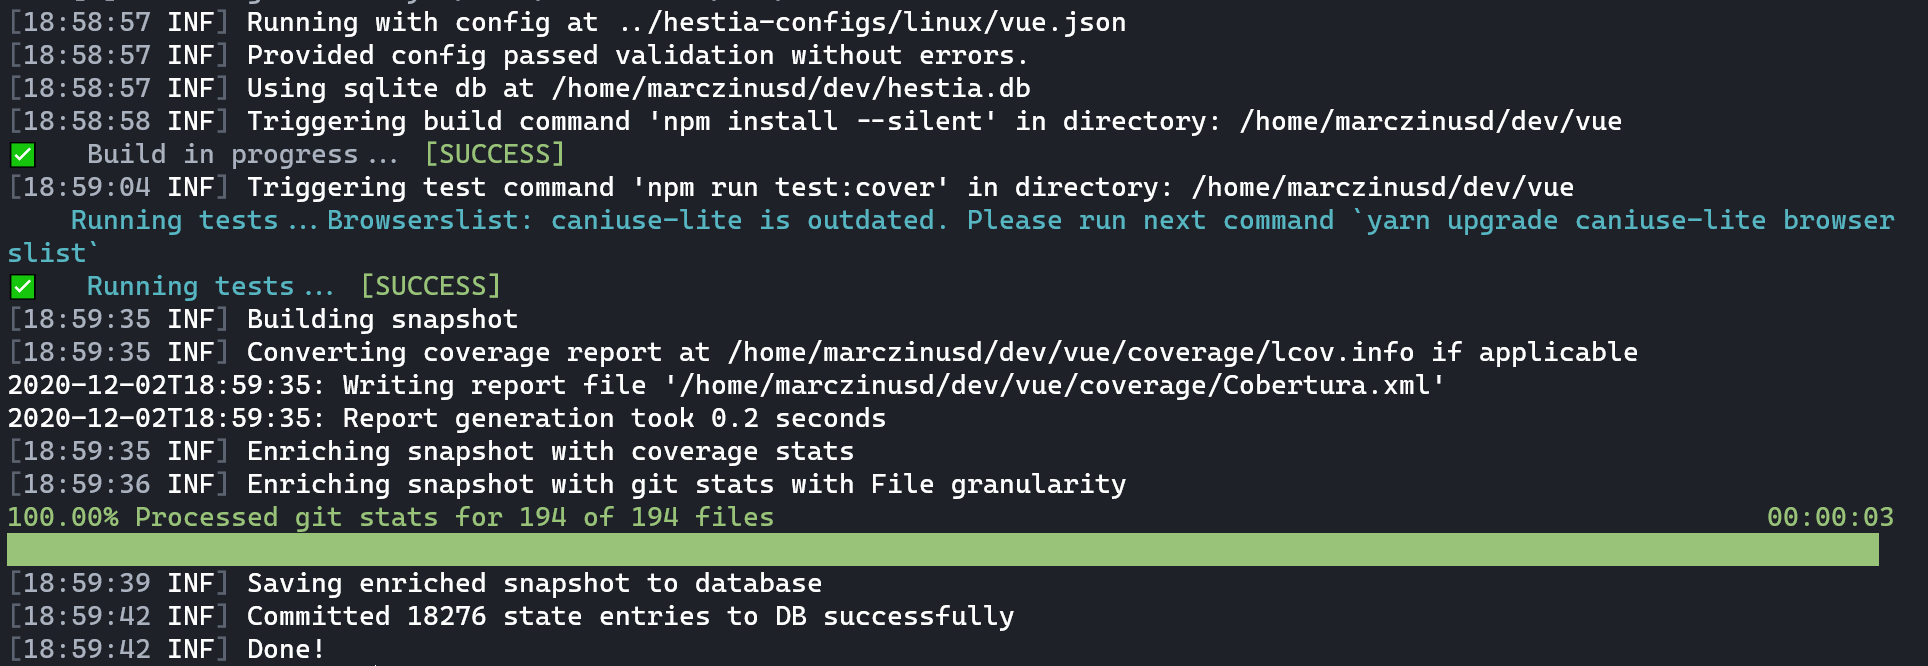
\includegraphics[width=1\textwidth]{images/hestia-console-run-vue.png}
    \caption{A konzolos futtató működés közben}
    \label{fig:console-runner-example}
\end{figure}

Fontos megjegyezni, hogy bár a konzolos futtató per pillanat csak egyedi snapshot analízis futtatásra lett felkészítve, maga a háttérben lévő modell képes repository-szintű analízisre is.

A repository-szintű analízis annyiban más, hogy paraméterül kap egy számot, ami a mintavételezési sűrűséget reprezentálja, azaz azt, hogy egy repository-ból hány snapshot-ot szeretnénk készíteni. Ugyan ez a fajta analízis is hasznos, a probléma jelenleg abban rejlik, hogy egy repository commit-jai nem egyenletesen oszlanak el az időben, így az implementáció, ami egyenletesen veszi a mintákat a commit-ok számának tekintetében, torzítani fogja az ereményeket a manuális mintavételezéssel szemben, ahol szempontnak számítanak többek között a szoftverfejleszétis mérföldkövet is.

\section{Web service}

A Hestia backend-jének utolsó nagy részét a ASP.NET Web API alapú, REST-es web service képezi. Ez tulajdonképpen arra hivatott, hogy a konzolos futtatás eredményeit szolgálja ki a külvilág számára könnyen emészthető módon, json formátumban. A service a következő endpoint-okat definiálja:
\begin{itemize}
    \item GET /snapshots: adjuk vissza az összes elérhető snapshot-ot, a snapshot teljes részletei nélkül
    \item GET /snapshots/\#snapshotId: adjuk vissza a megadott ID-hez tartozó snapshot részleteit
    \item GET /files/\#fileId: adjuk vissza a megadott ID-hez tartozó fájl részleteit
\end{itemize}

A service továbbá host-ol egy Swagger UI-t, ami dokumentálja és kipróbálhatóvá teszi az összes endpoint-ot. A service elindítása után a Swagger UI a \code{https://localhost:5001/index.html} címen érhető el.

\section{Hestia UI - Vékony kliens}

A webes kliens egy Angular 11-ben készült és szintén nagyban funkcionális és reaktív programozási koncepciókra épít az RXJS\footnote{https://github.com/ReactiveX/rxjs} segítségével, illetve modern state management-et implementál az Akita\footnote{https://github.com/datorama/akita} nevű könyvtár használatával. A webes kliens modellje megfelel a korábban definiált modellnek, TypeScript-ben implementálva.

A kliens képes megmutatni:
\begin{itemize}
    \item Az összes elérhető snapshot-ot
    \item A snapshot mögött lévő fájlokat a statisztikákkal párosítva, táblázatos formátumban
    \item A fájlok tartalmát sor-szintű statisztikákkal egy Monaco szövegszerkesztőben
    \item Snapshot-szintű statisztikákat grafikonokon ábrázolva
\end{itemize}

\begin{figure}[H]
    \centering
    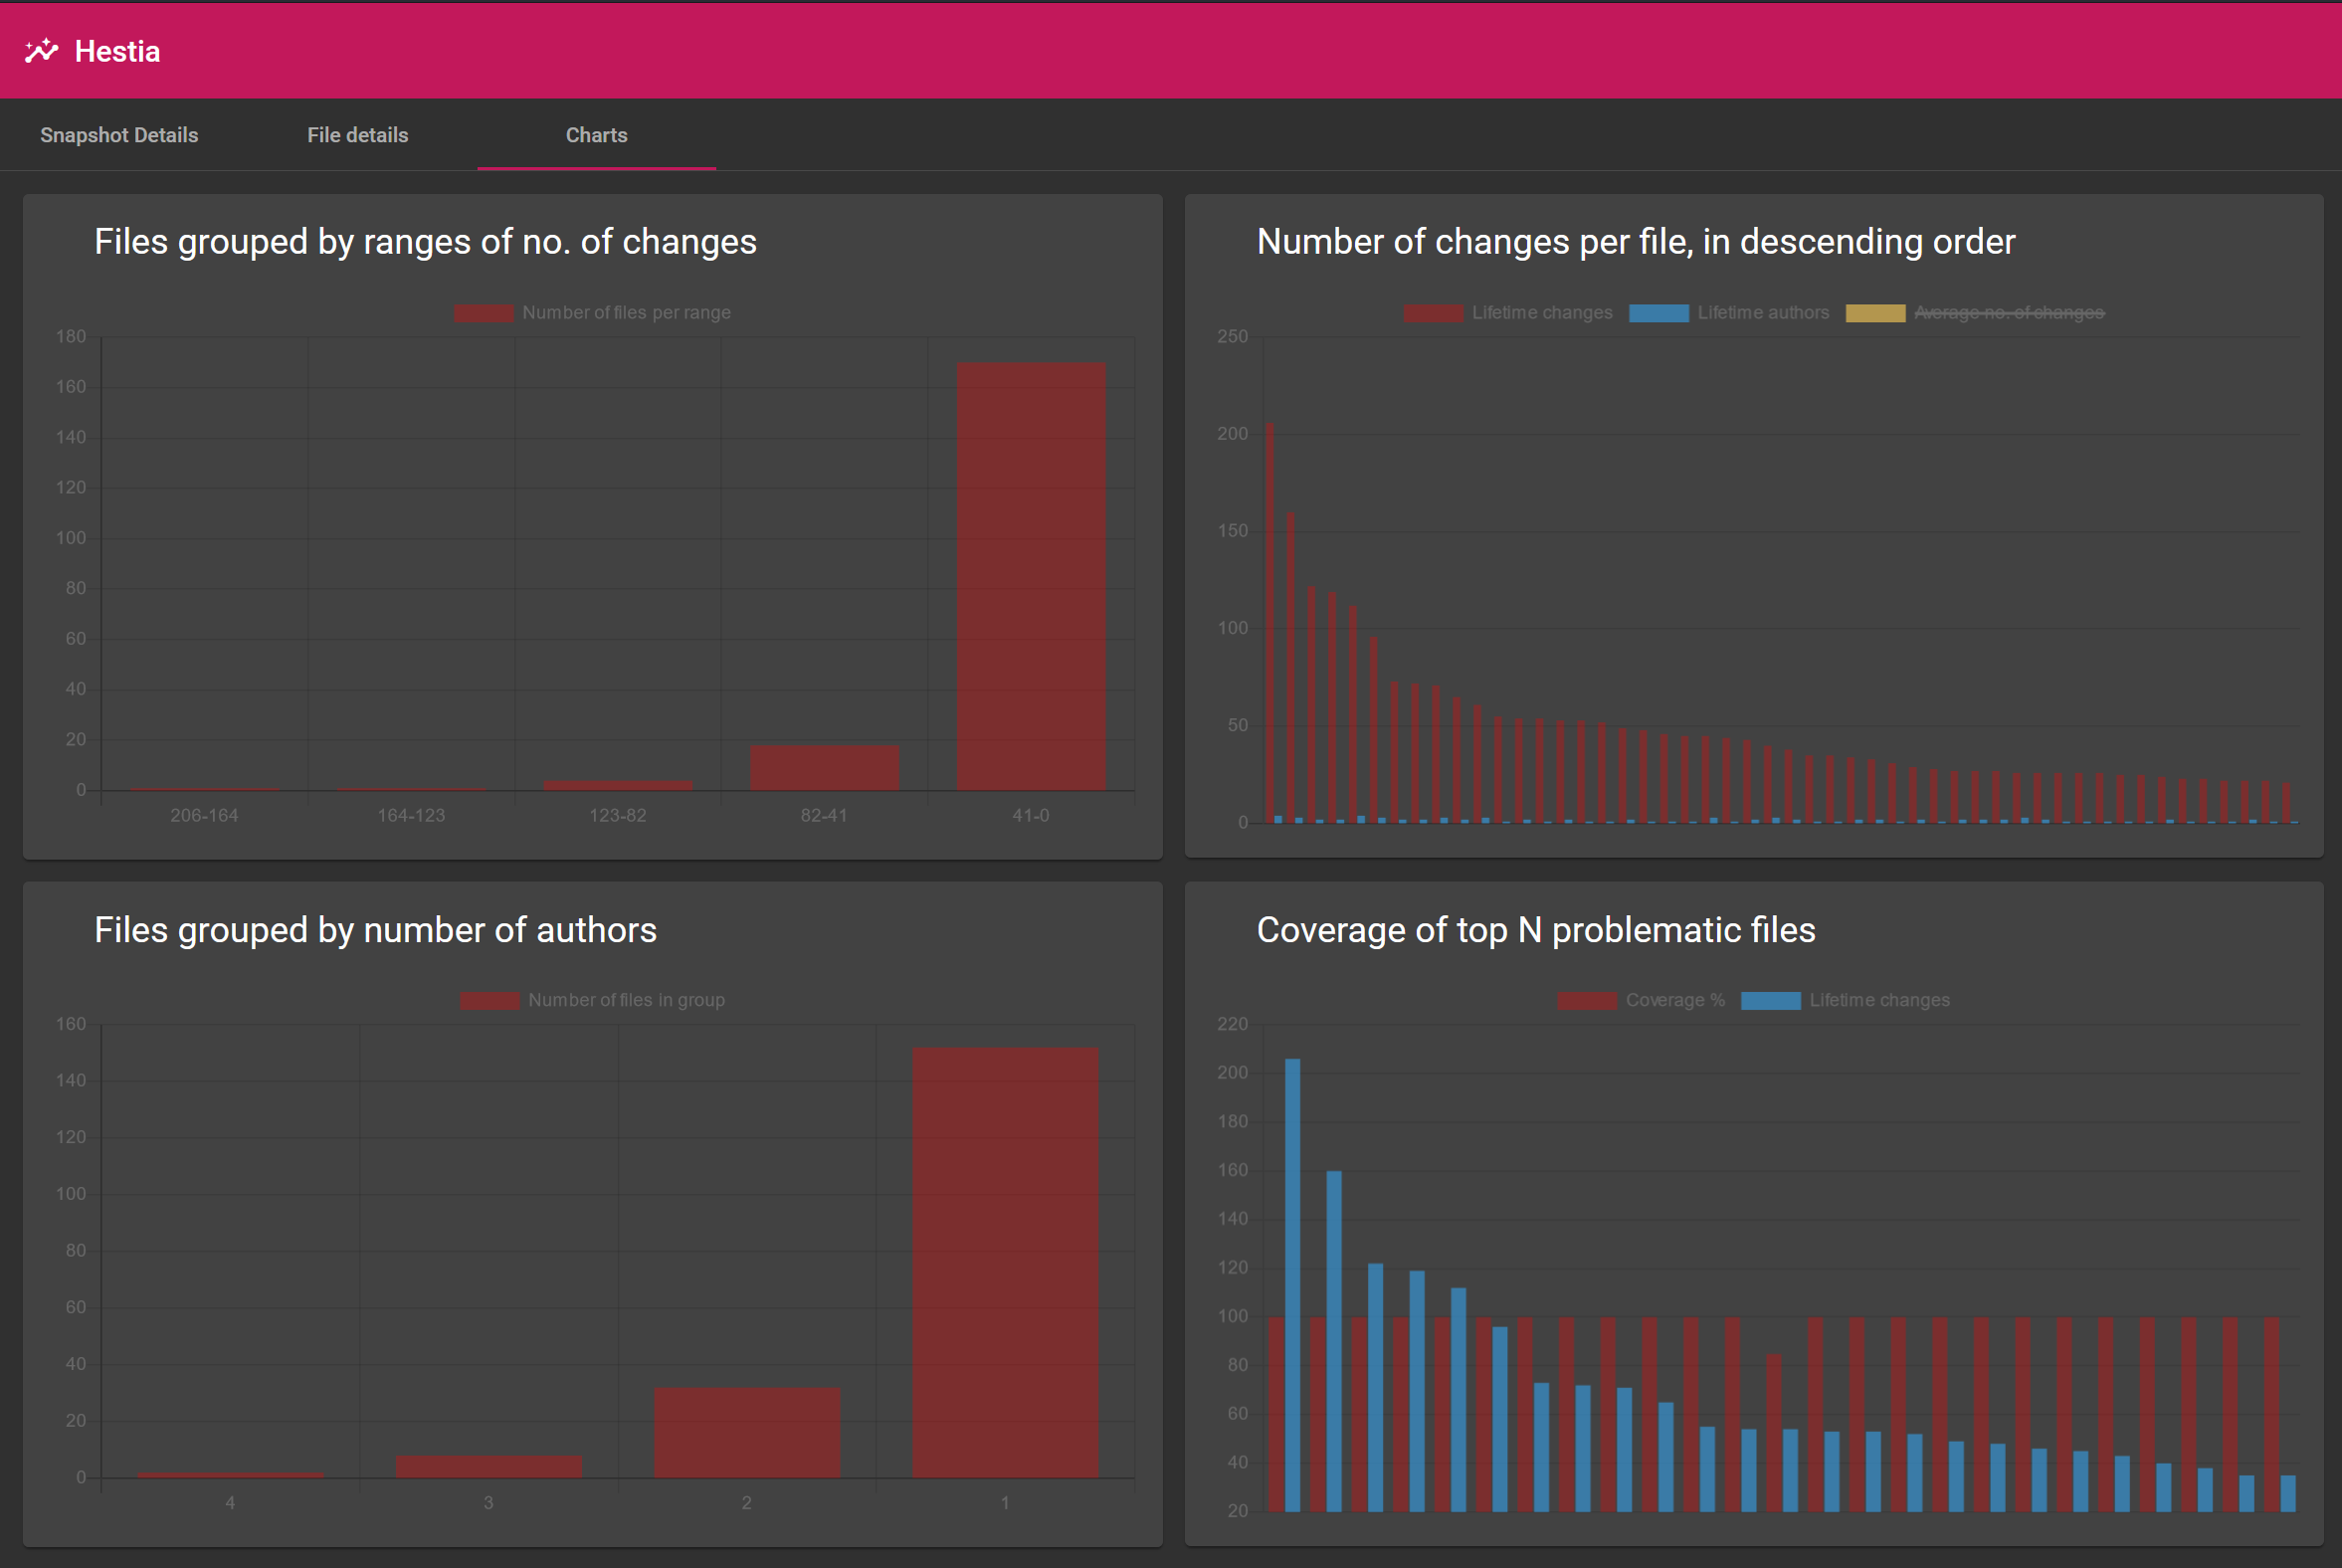
\includegraphics[width=1\textwidth]{images/hestia_charts.png}
    \caption{A vékony kliens által generált grafikonok}
    \label{fig:hestia-charts}
\end{figure}

\section{A program használata}

A .NET alapú konzolos futtató és web service használatának egyetlen előfeltétele, hogy a .NET 5 SDK\footnote{https://dotnet.microsoft.com/download/dotnet/5.0} telepítve legyen. A könnyebb futtatáshoz erősen ajánlott továbbá a GNU Make\footnote{https://www.gnu.org/software/make/} is, mert azzal elérhetővé válnak a dedikált build target-ek, amiket a továbbiakban részletezni fogok. Amennyiben a make nem áll rendelkezésre, akkor a projekt gyökerébem lévő makefile megfelelő build target-jének a parancsait kell sorrendben futtatni.

Első lépésben a forráskódot\footnote{https://github.com/marczinusd/hestia} git segítségével le kell tölteni, majd a projekt gyökerében állva a következő módon tudjuk futtatni a programot:

\begin{itemize}
    \item Analízis futtatása konzolon keresztül: \code{make run-console -{}- -{}-configPath "/path/to/config-file.json" }, ahol a konfigurációs fájl a korábban megadott formátumban van
    \item Web service indítása: \code{make run-webservice}
\end{itemize}

A webes kliens futtatásához egyedül egy telepített NodeJS-re van szükség. A forráskód\footnote{https://github.com/marczinusd/hestia-ui} letöltése után a projekt gyökerében állva ki kell adni az \code{npm install} parancsot, majd miután az lefutott az \code{npm start} fogja kiszolgálni a webes klienst a konzolon kiírt URL-en keresztül.
